% Same Storm, Different Boats: Generative AI and the Age Gradient in Hiring
% Economics Letters — body ≤2,000 words excl. references; abstract ≤100 words.
% LaTeX template: elsarticle (Elsevier)

\documentclass[preprint,12pt,authoryear]{elsarticle}

\usepackage[utf8]{inputenc}
\usepackage[T1]{fontenc}
\usepackage{amsmath,amssymb}
\usepackage{graphicx}
\usepackage{booktabs}
\usepackage{hyperref}
\usepackage{natbib}
\usepackage{setspace}
\usepackage{xcolor}
\usepackage{microtype}

% Set PDF metadata explicitly to avoid elsarticle frontmatter leaking
% internal tokens (\@corref, \cnotenum, \<def>) into the PDF string.
\hypersetup{
  pdftitle={Same Storm, Different Boats: Generative AI and the Age Gradient in Hiring},
  pdfauthor={Magnus Lodefalk and Lydia L\"othman and Michael Koch and Erik Engberg},
  pdfsubject={Generative AI and labour markets},
  pdfkeywords={Generative AI; Job postings; Labour demand; Employment composition; Monetary policy},
  hidelinks
}

% Path to figures
\graphicspath{{../figures/}}

\journal{Economics Letters}

\begin{document}

\begin{frontmatter}

\title{Same Storm, Different Boats: Generative AI and the Age Gradient in Hiring\tnoteref{version}}
\tnotetext[version]{This version: 18 September 2026. Latest version available at \url{https://www.ai-econlab.com/papers}.}

\author[oru,ratio]{Magnus Lodefalk\corref{cor}}
\ead{magnus.lodefalk@oru.se}
\author[oru]{Lydia L\"othman}
\author[au,kiel]{Michael Koch}
\author[oru,ratio]{Erik Engberg}

\cortext[cor]{Corresponding author}
\address[oru]{\"Orebro University School of Business, SE-701 82 \"Orebro, Sweden}
\address[ratio]{RATIO Institute, Stockholm, Sweden}
\address[au]{Department of Economics and Business Economics, Aarhus University, Denmark}
\address[kiel]{Kiel Institut f\"ur Weltwirtschaft, Germany}

\begin{abstract}
Whether generative AI or monetary tightening explains the post-2022 stock-price--job-postings divergence is debated. We study both margins in Sweden using full-population register data (2019--2025) and 4.9 million job advertisements (2020--2026). Using employer-level difference-in-differences and the seven-month gap between the Riksbank's first rate hike (April 2022) and the ChatGPT launch (November 2022), we find that the aggregate posting decline tracks monetary tightening; within employers, employment of workers aged 22--25 in AI-exposed occupations is 16 per cent lower after ChatGPT, concentrated among young women and operating through reduced hiring. The same within-employer decline appears in public job advertisements, whose coverage is independent of the register.
\end{abstract}

\begin{keyword}
Generative artificial intelligence \sep Job postings \sep Labour demand \sep Employment composition \sep Monetary policy
\JEL J23 \sep J24 \sep O33
\end{keyword}

\end{frontmatter}

% ══════════════════════════════════════════════════════════════════════════════
\section{Introduction}
% ══════════════════════════════════════════════════════════════════════════════

Since late 2022, US stock prices rose more than 70 per cent while job openings fell more than 30 per cent, prompting debate over whether generative AI or monetary tightening explains the divergence \citep{thompson2025scary}. Using ADP payroll data, \citet{brynjolfsson2025canaries} document a 16 per cent employment decline among young US workers in AI-exposed occupations, the ``canaries in the coal mine''; \citet{hosseini2025seniority} find a similar seniority gradient in US CV and job-posting data. Whether the pattern reflects AI or coincident monetary tightening, and whether it generalises beyond the US, remains open. In Sweden, the broad fall in postings tracks monetary tightening, whereas within employers high-AI-exposure occupations shifted away from workers aged 22--25 after ChatGPT, mainly through lower hiring.

We exploit a timing contrast that helps distinguish the channels: the Riksbank began raising rates in April 2022, seven months before ChatGPT launched in November 2022. If monetary tightening drives the differential posting decline, it should begin with the rate hike; if generative AI drives it, the decline should not appear before late 2022 and may emerge with adoption lags into 2023--2024. Using 4.6 million advertisements from Platsbanken (the Swedish Public Employment Service vacancy portal, 2020--2026), matched to the Dynamic AI Occupational Exposure (DAIOE) index \citep{engberg2024daioe}---an occupation-level index of exposure to generative AI---we decompose the aggregate posting decline by AI exposure. Postings across all exposure quartiles peak in mid-2022 and decline together through 2024, with at most a small additional drop in high-exposure occupations after ChatGPT.

We complement the posting evidence with population-register employment data and an employer-level difference-in-differences design \citep{brynjolfsson2025canaries}. Within the same employers, employment of workers aged 22--25 in high-AI-exposure occupations is 16.0 per cent lower than in less-exposed occupations after ChatGPT (95 per cent confidence interval (CI) [$-17.8$, $-14.1$]). The gradient is concentrated below age 30; the adjustment loads on the hiring margin, not on separations. Beyond the timing contrast, the contribution is to provide population-register evidence of an age-gradient adjustment outside the US, contrasting with the Finnish null in \citet{kauhanen2026youth}, which persists even when Swedish workers are reweighted to the Finnish industry-occupation mix. Because register occupation codes are assigned with a lag, we also reproduce the within-employer design on public job advertisements, where the employer identifier is recorded at publication and coverage does not depend on our data construction.


% ══════════════════════════════════════════════════════════════════════════════
\section{Data and empirical strategy}\label{sec:data}
% ══════════════════════════════════════════════════════════════════════════════

\paragraph{Job-posting margin} We use the full population of advertisements published on Platsbanken from January 2020 through June 2026. Each ad contains a publication date, a four-digit occupation code from the Swedish Standard Classification of Occupations (SSYK 2012), a vacancy count, a municipality, and an employer identifier. Of the 4{,}631{,}741 advertisements published in 2020--2025 we drop 4{,}951 without an occupation field and 40{,}615 duplicates, leaving 4{,}586{,}173; the 2026 half-year adds 289{,}601. No advertisement is lost to an invalid code, and the share carrying a valid SSYK code is 100.0 per cent in every month from 2022, against 99.0 and 99.3 per cent in 2020 and 2021 (Online Appendix~II.10). Of 400 occupations in the advertisements, 369 enter the regression sample; the 31 others are military and senior-manager codes for which the exposure index is undefined. Cells are occupation-by-month.\footnote{Historical bulk data (2020--2025) and the closed-quarter files for 2026 from \url{https://data.jobtechdev.se/annonser/historiska/}. Until 2007, private and local-government employers were legally required to post vacancies on Platsbanken \citep{cronert2021regulatory}; remaining sample-coverage details are in Online Appendix~II.4. Descriptive series are cut at December 2025 because the collection under-counts the two most recent months at any extraction date; the regressions use the closed-quarter files, which are complete through June 2026.}

We measure generative-AI exposure using the DAIOE index \citep{engberg2024daioe}, which maps AI benchmark capabilities to Swedish occupations at the SSYK 4-digit level. We use the 2023 cross-section of the percentile ranking for generative AI and classify occupations into quartiles, where Q4 is the most exposed.

The baseline specification is
\begin{equation}\label{eq:did}
\begin{split}
\ln(\text{postings}_{it}) = \alpha_i + \gamma_t &+ \beta_1 \cdot \text{PostRB}_t \cdot \text{High}_i \\
&+ \beta_2 \cdot \text{PostGPT}_t \cdot \text{High}_i + \varepsilon_{it},
\end{split}
\end{equation}
where $i$ indexes SSYK4 occupations, $t$ months, and $\alpha_i$ and $\gamma_t$ are occupation and month fixed effects. $\text{PostRB}_t = 1$ for $t \geq$ April 2022 (the Riksbank's first rate hike); $\text{PostGPT}_t = 1$ for $t \geq$ December 2022 (the first full month after ChatGPT's 30 November launch); $\text{High}_i = 1$ if occupation $i$ is in the top quartile of generative-AI exposure. Standard errors are clustered at the occupation level. The key test is whether the relative posting decline in high-exposure occupations begins with monetary tightening ($\hat\beta_1$) or with the advent of generative AI ($\hat\beta_2$).

\paragraph{Employment margin} {\sloppy For employment, we use monthly individual-level employer-declaration data (\emph{Arbetsgivardeklaration på individnivå}) from Statistics Sweden (SCB), hereafter the employer-declaration register. We link each worker to SSYK 4-digit occupation, age, and gender from the annual LISA register (Longitudinal Integration Database for Health Insurance and Labour Market Studies); together they cover the full population of employed individuals.\footnote{Both registers have been stable through the study period: the employer-declaration register since its 2019 introduction, and the SSYK 2012 classification used in LISA throughout.} We assign AI exposure from the DAIOE quartile of each worker's most recent occupation. Swedish university completion typically extends into the late twenties, so workers aged 22--25 proxy very-early-career employment (Online Appendix~III.1).\par}

For each age group $a$ we estimate
\begin{equation}\label{eq:emp_did}
\mathbb{E}[n_{f,q,t}] = \exp\!\left(\alpha_{f,q} + \delta_{f,t} + \gamma_1 \cdot \text{PostRB}_t \cdot \text{High}_q + \gamma_2 \cdot \text{PostGPT}_t \cdot \text{High}_q\right),
\end{equation}
where $f$ indexes employers, $q$ DAIOE quartiles, and $n_{f,q,t}$ counts age-group-$a$ workers at employer $f$ in quartile $q$ in month $t$, following \citet{brynjolfsson2025canaries}. Employer$\times$quartile fixed effects $\alpha_{f,q}$ absorb time-invariant compositional differences; employer$\times$month fixed effects $\delta_{f,t}$ absorb all firm-level time-varying shocks, so identification comes from within-employer recomposition across AI-exposure quartiles. Standard errors are clustered by employer$\times$quartile. The coefficient $\gamma_2$ is the age-group-specific analogue of $\beta_2$ in Equation~\eqref{eq:did}, and $\exp(\gamma_2)-1$ is a proportional change in employment. We estimate Equation~\eqref{eq:emp_did} by Poisson pseudo-maximum likelihood rather than by least squares on $\ln(n+1)$. Seventy per cent of cells are zero at ages 22--25, and the log-of-one-plus transform then returns no percentage change: its coefficient depends on the unit of the count \citep{chen2024logs}. Poisson accommodates the zeros and is consistent under the same conditional-mean assumption; $\ln(n+1)$ estimates are reported alongside (Online Appendix~III.6).


% ══════════════════════════════════════════════════════════════════════════════
\section{Results}\label{sec:results}
% ══════════════════════════════════════════════════════════════════════════════
Figure~\ref{fig:scary} shows the Swedish stock-price--job-postings divergence. The OMXS30 (the Stockholm large-cap index) reached 175 per cent of its February 2020 level by early 2026, while job postings across all AI-exposure quartiles declined together from the Riksbank rate hike in April 2022. The divergence opens seven months before ChatGPT, coinciding with monetary tightening. The pattern is identical with the broader OMXSPI All-Share index (Online Appendix~II.2).

\begin{figure}[ht!]
\centering
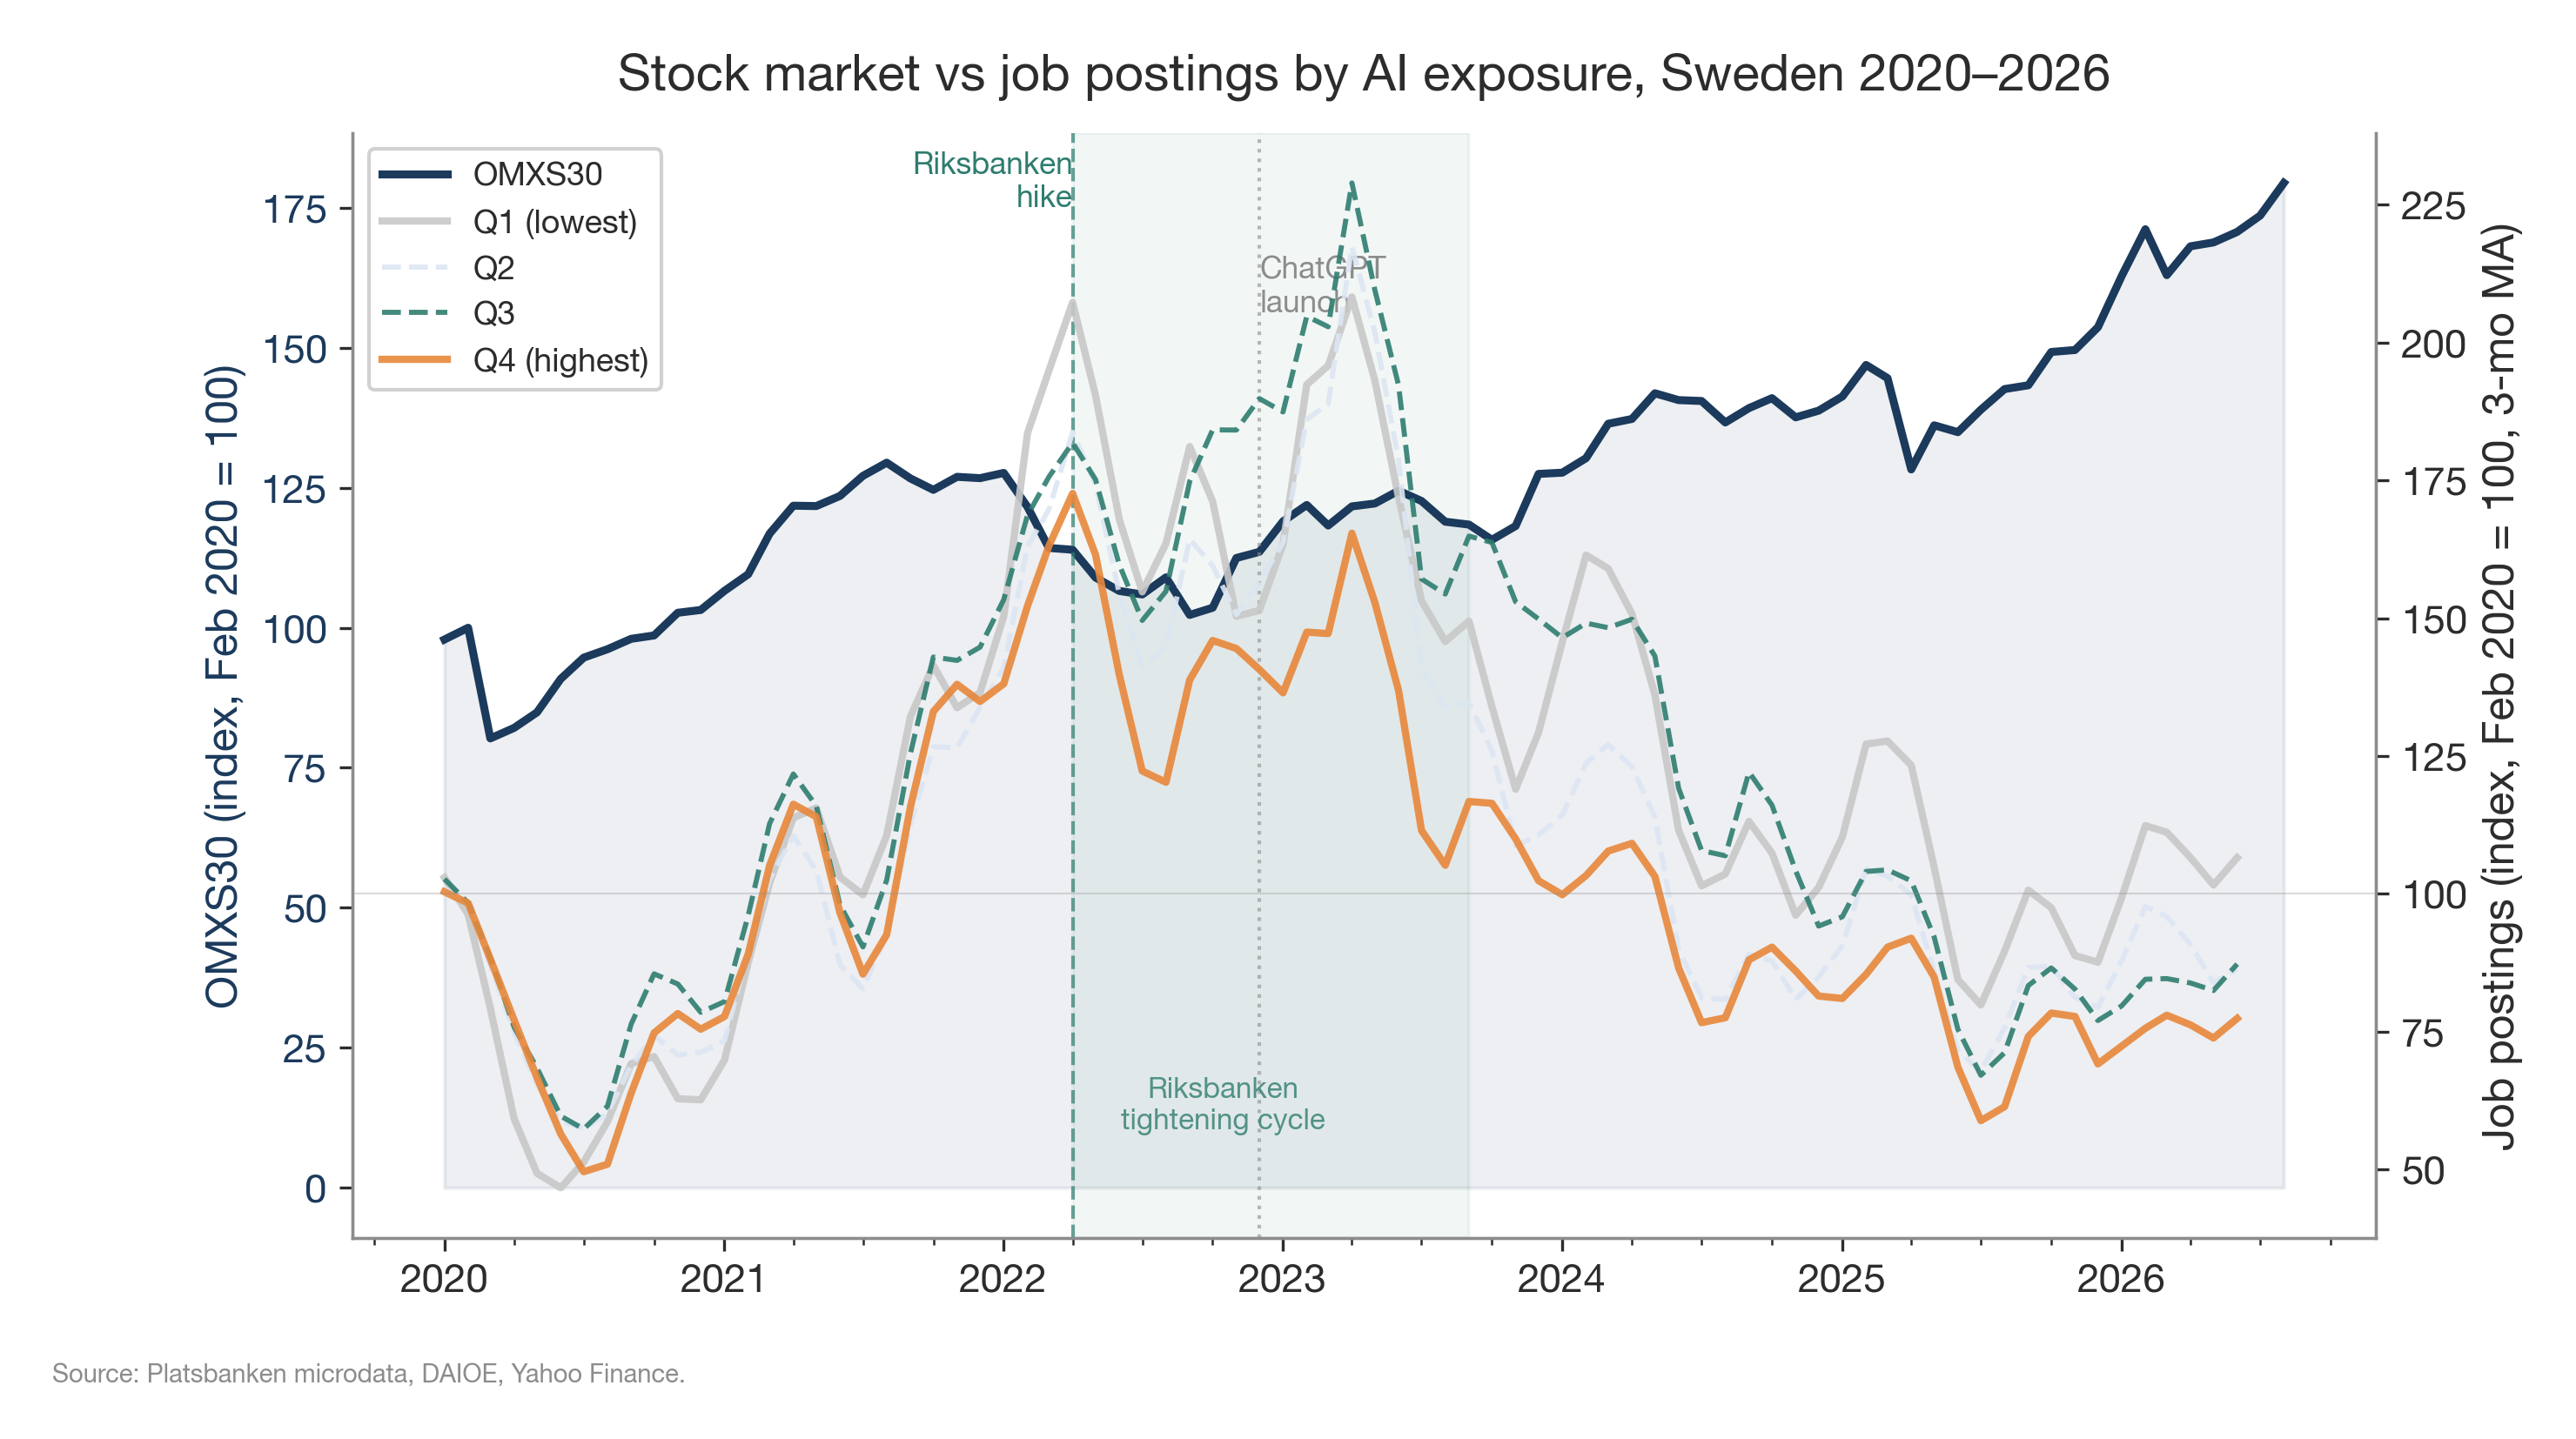
\includegraphics[width=\textwidth]{fig1_scary_chart.png}
\caption{Stock market vs job postings by AI-exposure quartile, Sweden 2020--2026. Daily OMXS30 closing prices (Yahoo Finance) are resampled to monthly averages and indexed to 100 at February 2020 (left axis); Platsbanken posting index by generative-AI exposure quartile is shown on the right axis. Vertical lines mark the Riksbank's first rate hike (April 2022) and the ChatGPT launch (November 2022).}
\label{fig:scary}
\end{figure}

Estimating Equation~\eqref{eq:did} through June 2026, we estimate the rate-hike interaction precisely at $\hat\beta_1 = -0.127$ (95 per cent CI [$-0.203$, $-0.052$]; $p < 0.01$), while the post-ChatGPT interaction is small and statistically indistinguishable from zero, $\hat\beta_2 = -0.059$ (95 per cent CI [$-0.134$, $+0.016$]; $p = 0.12$). Poisson estimation of the same specification gives $-0.129$ ($p = 0.01$) and $-0.060$ ($p = 0.15$), and adding occupation-group$\times$calendar-month fixed effects moves both coefficients by less than 0.004, so neither the transform nor seasonality carries the result (Online Appendix~II.9, II.11). AI exposure is uncorrelated with revealed monetary-policy sensitivity ($r = 0.04$, $p = 0.51$; Online Appendix~II.7), consistent with the channels being distinct.

The employment margin shows a different pattern. Figure~\ref{fig:canaries} plots the raw monthly employment series by age group and AI-exposure quartile (3-month moving average; the unsmoothed series is in Online Appendix~III.1). Employment of workers aged 22--25 in high-AI-exposure occupations diverges from the comparison groups during 2024 and the gap widens through mid-2025; the aggregated 26+ series is comparatively stable, masking heterogeneity within older bins.

\begin{figure}[ht!]
\centering
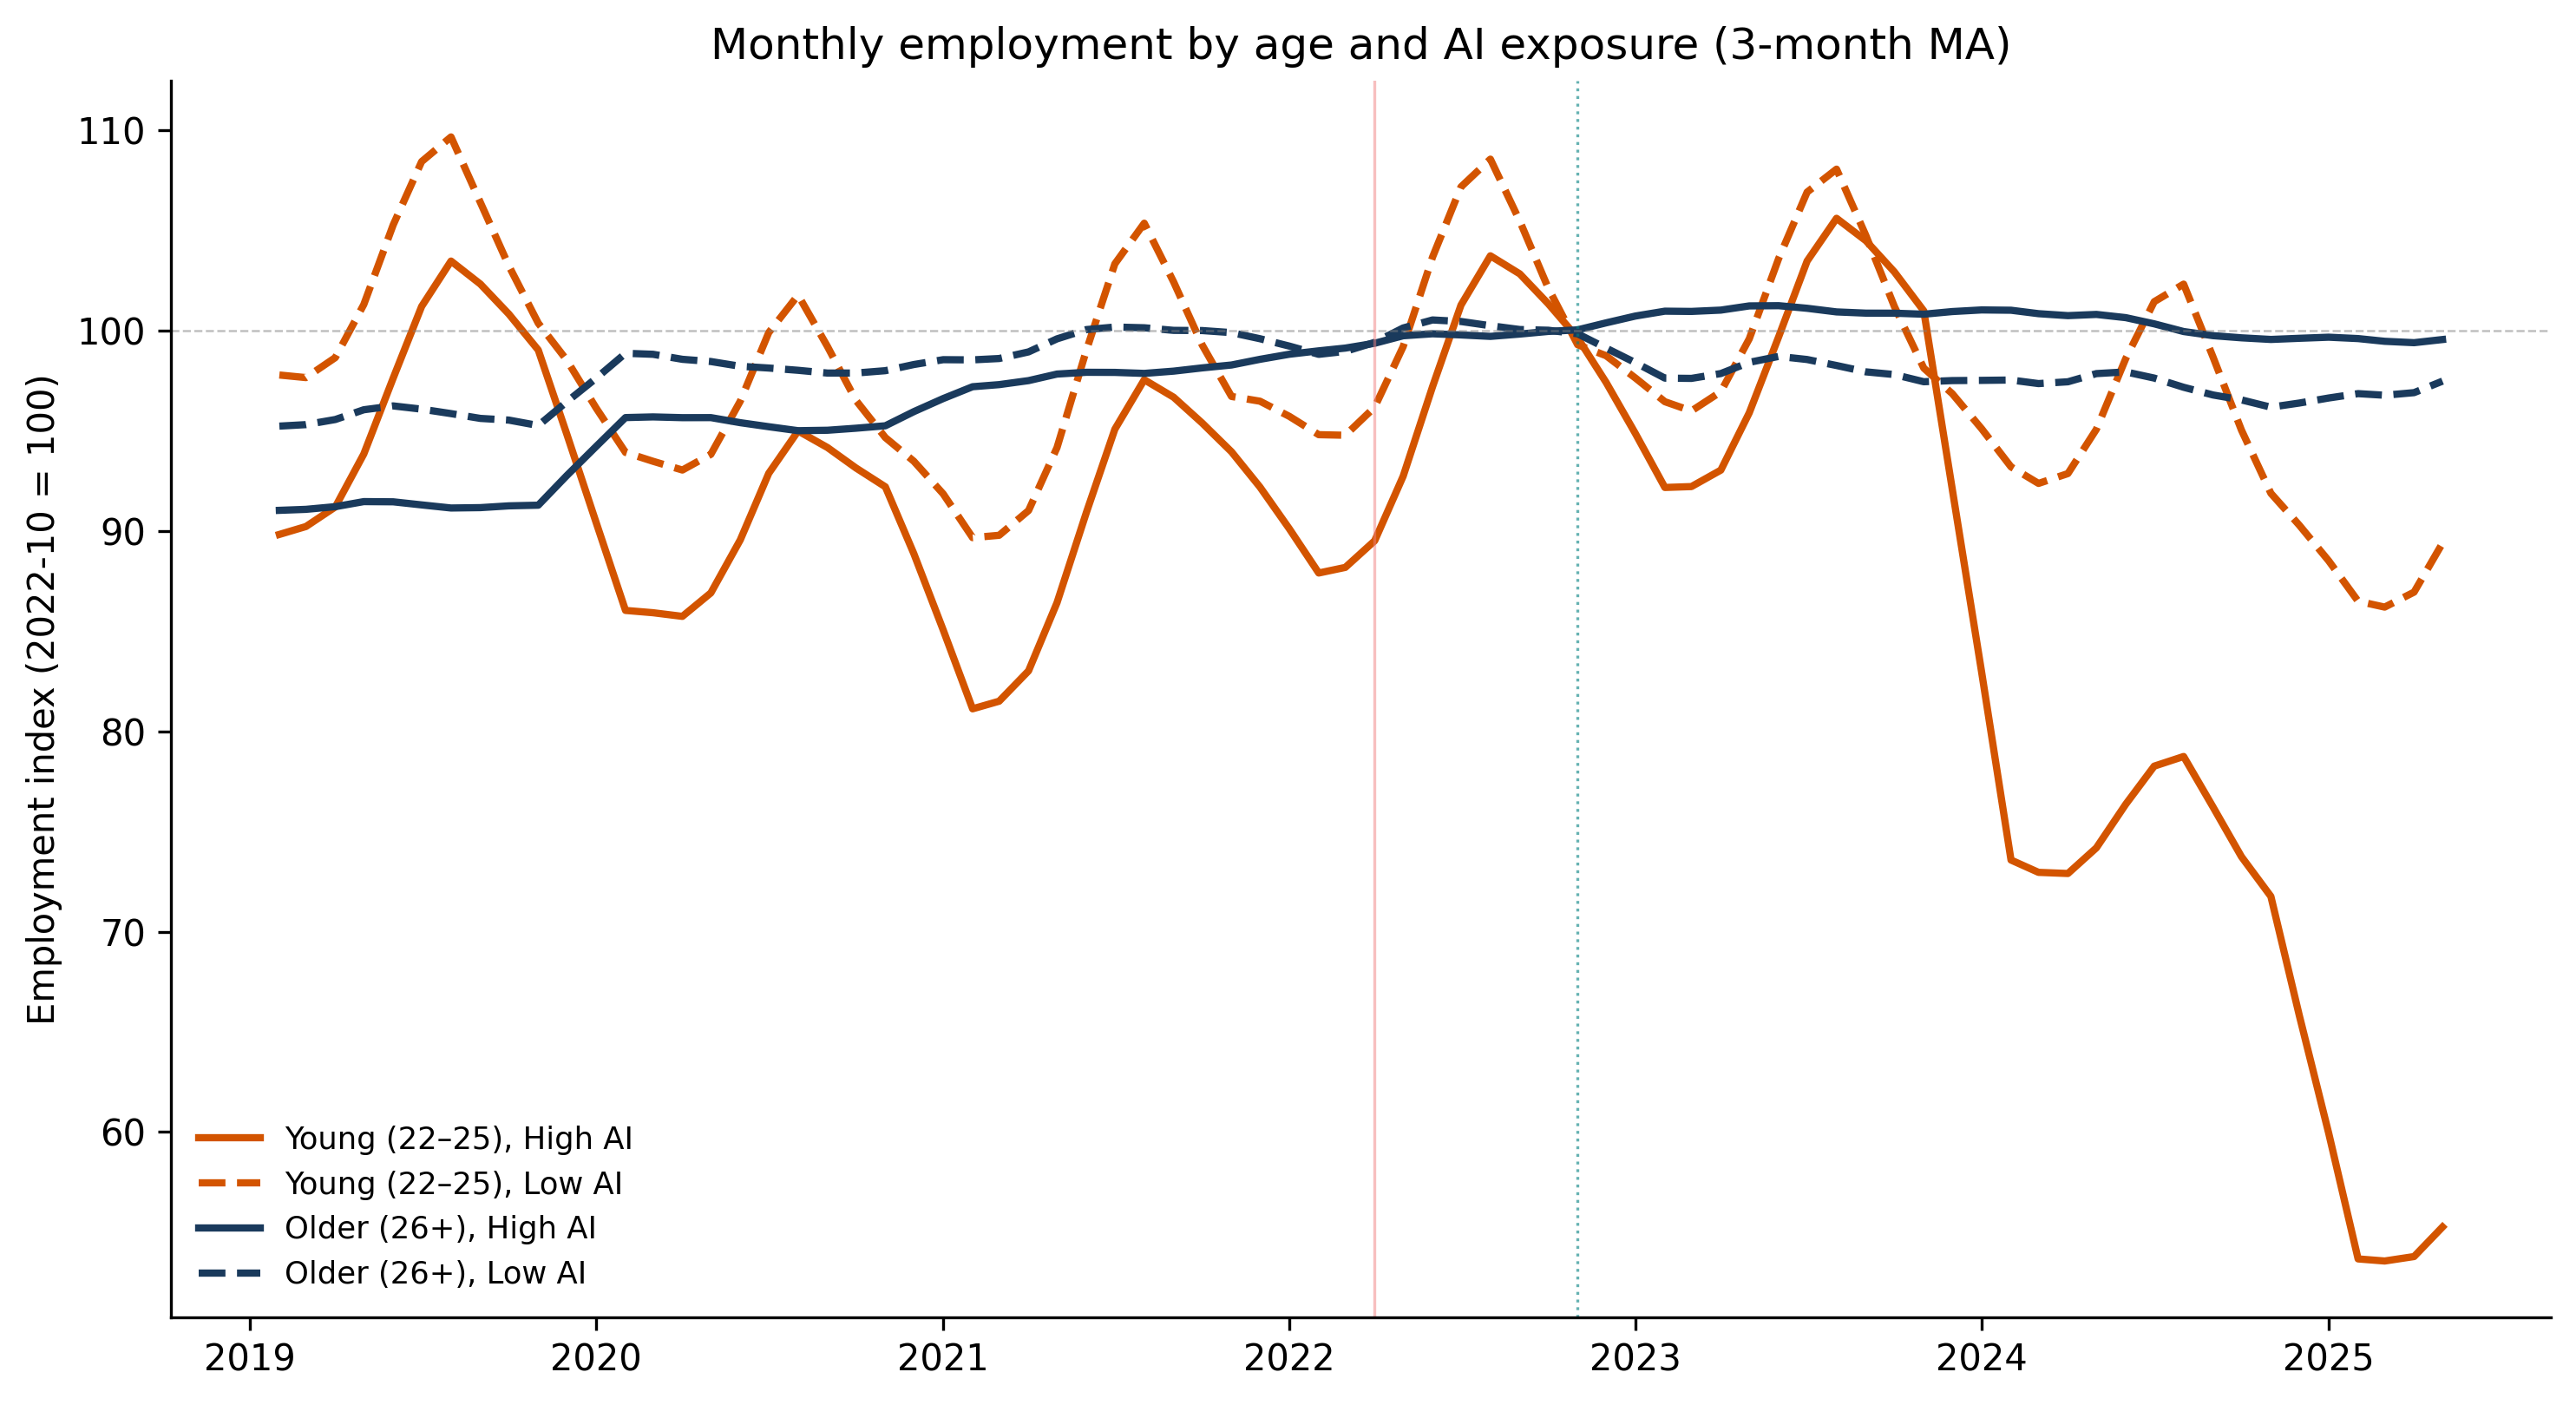
\includegraphics[width=\textwidth]{fig2_mona_canaries_ma3.png}
\caption{Monthly employment by age group and AI exposure, Sweden 2019--2025 (3-month moving average). Employer-declaration register data indexed to October 2022 = 100. Young (22--25) versus older (26+) workers, split by AI-exposure quartile (DAIOE). Vertical lines mark the Riksbank's first rate hike (April 2022) and the ChatGPT launch (November 2022).}
\label{fig:canaries}
\end{figure}

Our headline estimand is the pooled post-ChatGPT coefficient for ages 22--25. Within the same employers, employment in top-quartile AI-exposed occupations is 16.0 per cent below less-exposed occupations after ChatGPT ($\hat\gamma_2 = -0.174$, SE 0.011; 95 per cent CI [$-17.8$, $-14.1$]). The $\ln(n+1)$ specification gives $-0.010$ (95 per cent CI [$-0.014$, $-0.006$]) on the same cells; the two estimators agree on sign, significance and age profile, and the gap in magnitude is the scale difference the transform induces (Online Appendix~III.6).

Figure~\ref{fig:age_gradient} shows the half-year event study for the same specification. The path is flat through 2023, breaks at the first half of 2024 ($-0.283$, SE 0.015) and reaches $-0.588$ (SE 0.026) by the first half of 2025. Two qualifications belong with it. Pre-period deviations are small but not all zero, the largest being $-0.051$ in the second half of 2021, so the pre-trend is not clean in the Poisson specification as it was in logs. More importantly, the 2024 break coincides with the point from which an increasing share of workers carries an occupation code from an earlier register year, so the dynamic path mixes a real effect with a mechanical one.
% TODO(45): insert the as-of backtest number here -- the artificial coefficient
% obtained by imposing 2024-25 staleness on the fully covered 2019-2023 panel.
% Until it lands, the pooled coefficient is the quantitative claim and the event
% study is shown for timing only. See notes/frozen-cohort-reconciliation_2026-09-06.md.
We therefore treat the pooled coefficient as the magnitude and the event study as evidence on timing, and quantify the mechanical component directly below.

The decline operates primarily through the hiring margin. In the same specification, the hires coefficient for ages 22--25 is $\hat\gamma_2^H = -0.0051$ (95 per cent CI [$-0.0061$, $-0.0041$]; $p < 0.001$), while the separations coefficient is one quarter as large in absolute terms ($\hat\gamma_2^S = -0.0012$, 95 per cent CI [$-0.0020$, $-0.0004$]; $p < 0.01$). Sweden's last-in-first-out employment-protection legislation constrains separations of incumbents, so exposed employers reduce entry hiring rather than dismissing staff (Online Appendix~III.3). This pattern is consistent with generative AI compressing codified, routine entry-level tasks rather than displacing established workers.
% TODO(41): incumbents vs new person-employer matches. The coverage-immune cohort
% (script 42) declines on its own, which the hiring-only reading does not predict,
% so "primarily" may need to become "at entry, with reallocation of young
% incumbents growing over 2024-25". Do not harden this sentence before 41 reports.

The age profile is sharply concentrated below age 30. The gradient extends to ages 26--30, where employment is 5.2 per cent lower (95 per cent CI [$-6.5$, $-3.8$]), a third of the effect at 22--25 (Online Appendix~III.2). Effects for ages 31--49 are essentially zero. The 50+ estimate is positive but small ($+2.4$ per cent, 95 per cent CI [$+1.6$, $+3.1$]) and disappears under the \citet{eloundou2024gpts} exposure score (Online Appendix~II.5, III.7). Population-level employment remains broadly stable, consistent with occupational reallocation rather than net job destruction. The 22--25 result strengthens in the long-tenured subsample, ruling out staleness in occupational coding as a driver (Online Appendix~III.8).

Two further pieces of evidence do not depend on how we construct the register panel. From January 2021 the employer's organisation number is recorded in 99 per cent of advertisements, so the within-employer design runs on the postings themselves, with the same two fixed effects, on 12{,}141 identifying employers through June 2026. The rate-hike interaction is zero ($+0.004$, $p = 0.72$); the post-ChatGPT interaction is $-0.158$ ($p < 0.001$), $-0.180$ excluding staffing agencies and public employers, and $-0.196$ on entry-level advertisements, whose event study deepens to $-0.47$ by 2026 (Online Appendix~V). That identifier is recorded at publication, so no occupation-code lag can generate the pattern. In Statistics Sweden's published aggregates, coded by the agency and not by us, 16--24 is also the only age band whose top-quartile gap falls by 2024, while every older band rises (Online Appendix~III.9).

The timing also does not fit a monetary explanation. The Riksbank began cutting rates in May 2024, and the differential decline deepens through 2024 and 2025, after easing had started.

The decline is concentrated among young women, in the $\ln(n+1)$ specification: $\hat\gamma_2 = -0.016$ (95 per cent CI [$-0.020$, $-0.012$]) for women aged 22--25, versus $-0.007$ (95 per cent CI [$-0.013$, $-0.001$]) for men, with a triple-difference $p < 0.01$ (Online Appendix~III.5). Reweighting women's occupations to men's narrows the gap by two-fifths (Online Appendix~III.5).
% TODO(48): the gender split and the hires/separations decomposition are still
% ln(n+1) estimates from the submitted round, now that Poisson is primary. Script
% 48 re-runs both in Poisson so the paper does not mix estimators. Until it
% reports, these two paragraphs state the estimator explicitly.

\begin{figure}[ht!]
\centering
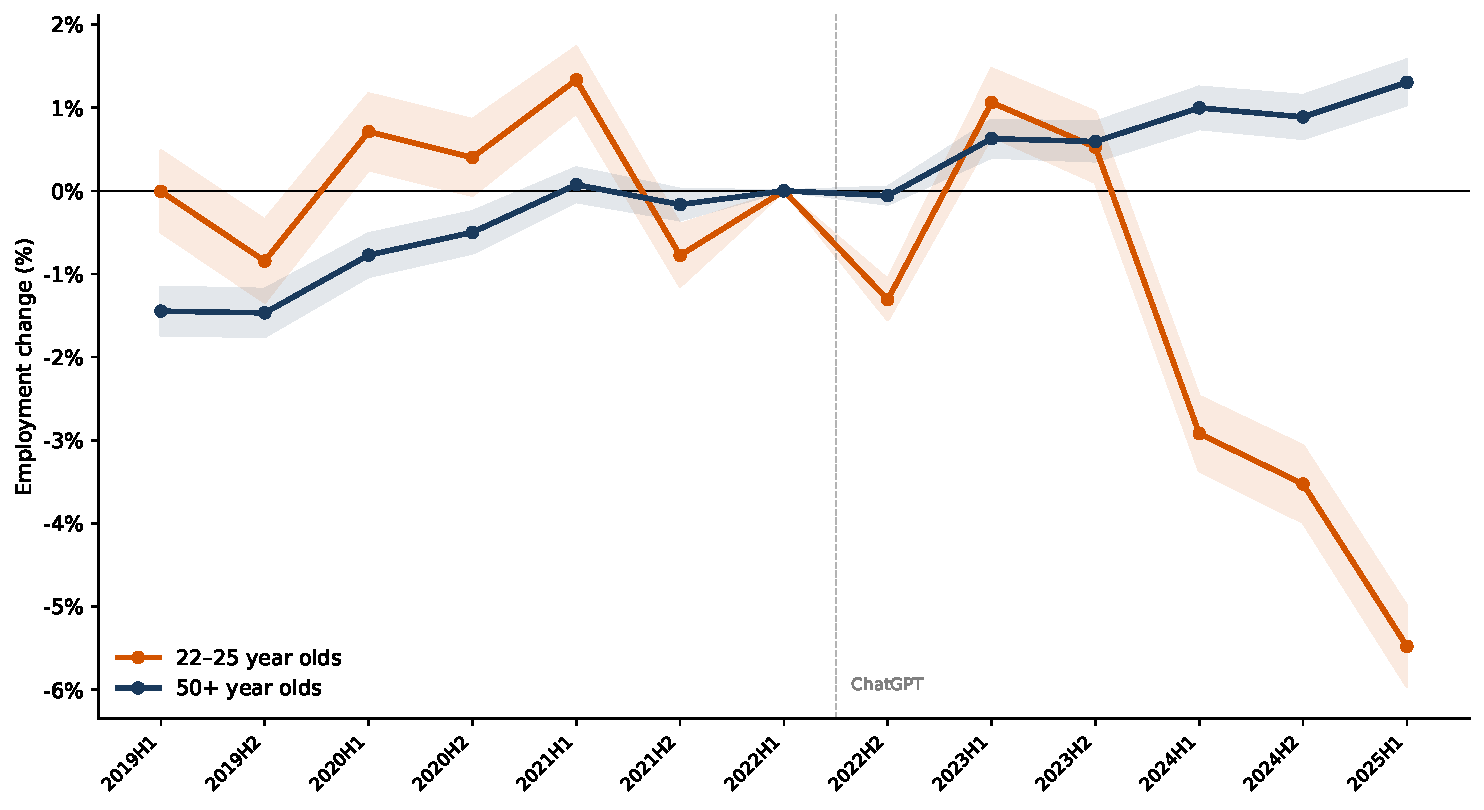
\includegraphics[width=\textwidth]{fig3_event_study_main.pdf}
\caption{Event study of employment effects by age group and AI exposure, ages 22--25 and 50+. Coefficients from employer-level regressions with employer$\times$quartile and employer$\times$month fixed effects, half-year periods, reference: first half of 2022. Shaded areas show 95 per cent confidence intervals. The dashed line marks the ChatGPT launch (November 2022). Coefficients from the log specification approximate percentage changes. All six age groups appear in Online Appendix~III.2.}
\label{fig:age_gradient}
\end{figure}


% ══════════════════════════════════════════════════════════════════════════════
\section{Conclusion}\label{sec:conc}
% ══════════════════════════════════════════════════════════════════════════════

The age gradient is consistent with generative AI substituting for codified, routine entry-level tasks while complementing the tacit, experiential expertise of senior workers \citep{acemoglu2019automation,acemoglu2026proworker}. Adjustment loads on the hiring margin, consistent with Sweden's incumbent-protection legislation. The finding survives in three data constructions whose coverage properties differ: the register panel, public job advertisements at the employer level, and the statistical agency's own published aggregates. We do not directly observe employers' AI adoption, so unobserved organisational changes correlated with exposure cannot be ruled out, and occupation codes in the register are assigned with a lag, which is why the paper measures that lag's contribution rather than assuming it away. If the pattern persists, the displacement of entry-level cohorts raises a longer-term skill-formation concern; transition pathways and junior-role redesign deserve attention.

% ══════════════════════════════════════════════════════════════════════════════
% Elsevier-required declarations
% ══════════════════════════════════════════════════════════════════════════════

\section*{Declaration of competing interest}
The authors declare no competing interests.

\section*{Declaration of generative AI and AI-assisted technologies in the manuscript preparation process}
During the preparation of this work the authors used Claude (Anthropic) to assist with code development, data processing, and editorial suggestions. After using this tool, the authors reviewed and edited the content as needed and take full responsibility for the content of the published article.

\section*{Funding}
This work was supported by the Torsten S\"oderberg Foundation (grants E46/21, ET3/23) to Lodefalk, and by WASP-HS (grant 805) to Lodefalk, L\"othman and Engberg. The funders had no role in study design, data analysis, manuscript preparation, or the decision to submit for publication.

\section*{Data availability}
{\sloppy
Platsbanken job advertisements are publicly available under a CC0 licence (\url{https://data.jobtechdev.se/annonser/historiska/}; \url{https://jobstream.api.jobtechdev.se}). The employment analysis uses confidential individual-level administrative microdata from Statistics Sweden (SCB), accessed via the secure MONA platform under ethical approvals listed below; access procedures are documented in Online Appendix~IV.1. All replication code is publicly available at \url{https://github.com/Magnus-L/canaries-sweden}; an archived release is referenced in the Online Appendix.\par}

\section*{Acknowledgements}
We thank Lars Hultkrantz, Sune Karlsson, and participants at workshops and seminars at AISCAF, and the Swedish Public Employment Service for helpful comments. Ethical approvals from the Swedish Ethical Review Authority (Etikpr\"ovningsmyndigheten): Dnr 2021-05040, 2022-03330-02, 2024-01714-0, 2025-04205-02.

% ══════════════════════════════════════════════════════════════════════════════
\bibliographystyle{elsarticle-harv}
\bibliography{references}

\end{document}
